\chapter{Программная реализация}

\section{Модель}

В качестве нейронной сети для сегментации сигнала была выбрана модель типа
"UNet". Выбор пал на нее, так как уже были работы, где она себя хорошо
зарекомендовала в схожей задаче \cite{victor}. В целом, это достаточно похожая
на оригинал одномерная версия модели. Однако не обошлось и без модификаций:

\begin{enumerate}

	\item Паддинг: для сохранения размера вектора при свертках используется
	      паддинг с зеркальным заполнением. Так же это позволяет получить равный по
	      размеру входу выход.

	\item Upsample: вместо обратных сверток на этапе восстановления
	      используется upsample, это необучаемая часть нейросети, поэтому обучение и
	      предсказание занимает заметно меньше времени.

\end{enumerate}

Сама модель состоит только из сверток, pooling слоев и слоев upsample, то есть
не включает в себя полносвязные слои. Можно выделить две части: ``спуск'' и
``подъем''. Каждый слой спуска состоит из двух последовательных сверток и слоя
max pool. Слой же подъема почти в точности повторяет спуск с тем отличием, что
выполняет обратную операцию, в связи с чем вместо max pool использует upsample.
Так же в архитектуре присутствуют остаточные связи, они соединяют
соответствующие части спуска и подъема посредством конкатенации тензоров.
Наглядно нейросеть изображена на рис. \ref{fig:unet}.

\begin{figure}[!htb]
	\centering
	\caption{Архитектура нейронной сети UNet}
	\includegraphics[width=\textwidth]{unet.png}
	\label{fig:unet}
\end{figure}


\section{Обучение}

Обучение нейронной сети производилось на компьютерах со следующими характеристиками:

\begin{enumerate}
	\item GPU: Nvidia GeForce RTX3070 (8Gb видеопамяти)
	\item RAM: 32Gb
	\item CPU: Intel Core i5 (6 ядер x 2.5 Ггц)
\end{enumerate}

В качестве метода оптимизации использовался adam (как один из самых продвинутых
методов стохастического градиентного спуска \cite{adam}) в паре с milestone шедуллером.

\subsection{Отслеживание экспериментов и метрик}

Благодаря тому, что в стеке используемых технологий есть язык программирования
Python, открывается возможность использования разнообразных библиотек для
удобства отслеживания экспериментов. В данном случае была выбрана библиотека
mlflow. Использовалась она для хранения информации о параметрах эксперимента,
таких как, например, learning rate, test fold, файл с реализаций нейронной
сети, loss, а так же для отслеживания метрик моделей (см. рис.
\ref{fig:mlflow-metrics}). В качестве такой метрики была loss функция. Она
записывалась каждый пакет и каждую эпоху.

\begin{figure}[!htb]
	\centering
	\caption{Пример отображения метрик для эксперимента в mlflow}
	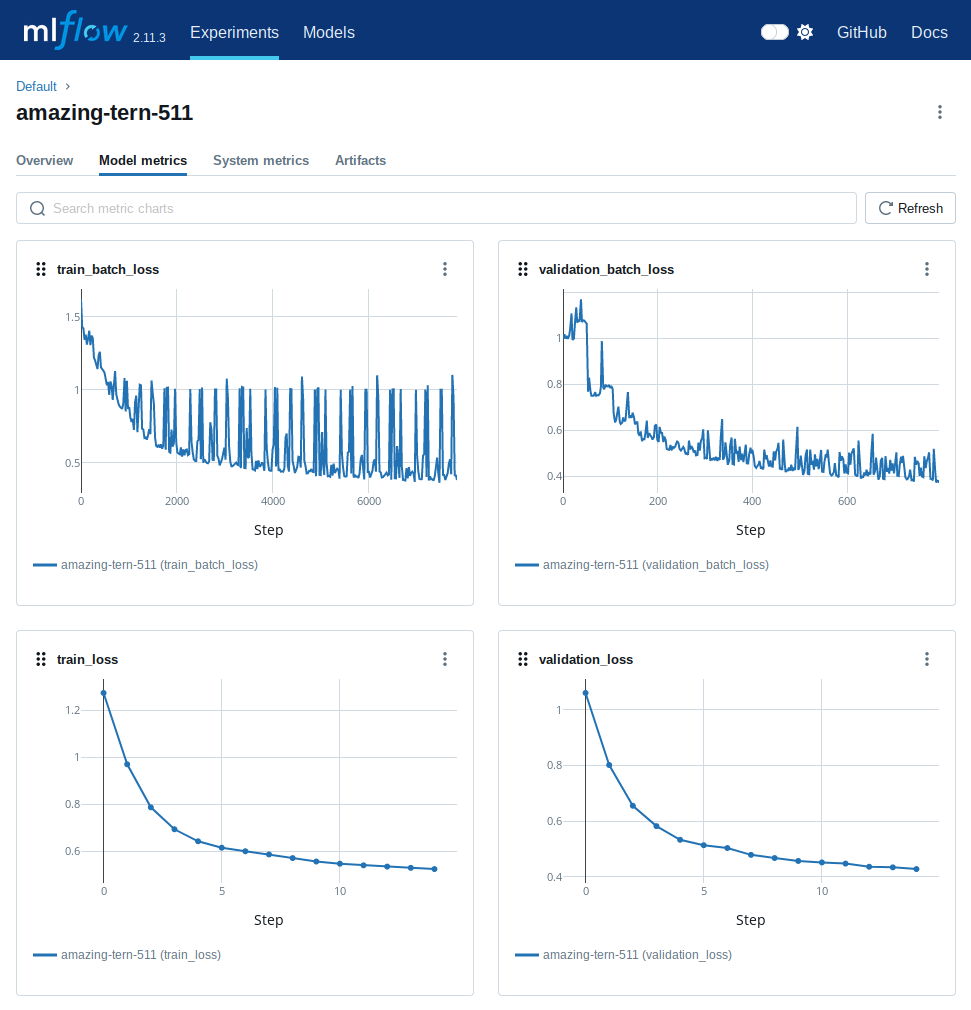
\includegraphics[width=\textwidth]{mlflow-metrics.png}
	\label{fig:mlflow-metrics}
\end{figure}


\subsection{Кросс валидация}
Так как в нашем распоряжении было не много размеченных данных, для исключения
переобучения использовалась кросс валидация. Как было описано ранее, предметным
специалистом были предоставлены примерно одинаковые по продолжительности записи
с разных экспериментов, в связи с чем было логично сделать разбиение на группы
именно по ним. Таким образом, всего у нас получилось 8 групп --- по 1 на
валидацию и тестирование и по 6 на обучение. Всего производилось 8
экспериментов (по одному на уникальную тестовую группу). Валидационная группа
выбиралась случайным образом. Метрики замерялись после обучения на тестовой
группе. В качестве финальной метрики бралось среднее от всех экспериментов.

\section{Предсказание}

\subsection{Постобработка}
Сырой выход модели представляет из себя тензор таких же размеров, что и вход,
содержащий для каждой точки входа вероятность наличия активации в ней. Однако
нас интересуют конкретные активации.

\section{Подсчет метрик}

После получения предсказания встает вопрос о подсчете метрик, ведь при прямом
сравнении, метки с предсказания и с разметки могут быть смещены относительно
друг друга, например, на несколько сэмплов. С учетом пожеланий предметного
специалиста, для исследований которого предоставлялось разметка, было решено
считать истинно положительной активацию, которая была предсказана с точностью
до 5 сэмплов.

Таким образом алгоритм подсчета выглядел следующим образом:

Для подсчета TP и FP производилась итерация по активациям предсказания. В
окрестности в 5 сэмплов от каждой метки производился поиск наличия таковой в
исходной разметке. В случае положительного результата предсказание считалось
как TP, иначе --- FP. Для подсчета FN итерация происходила по активациям исходной
разметке, а поиск --- по предсказанию. Активация считалась FN в случае
отсутствия результатов поиска в окрестности истинной метки. Наглядно это
изображено на рис. \ref{fig:metrics} (желтым выделен сигнал, по меткам которого
происходит итерация).

\begin{figure}[!htb]
	\centering
	\subfigure[]{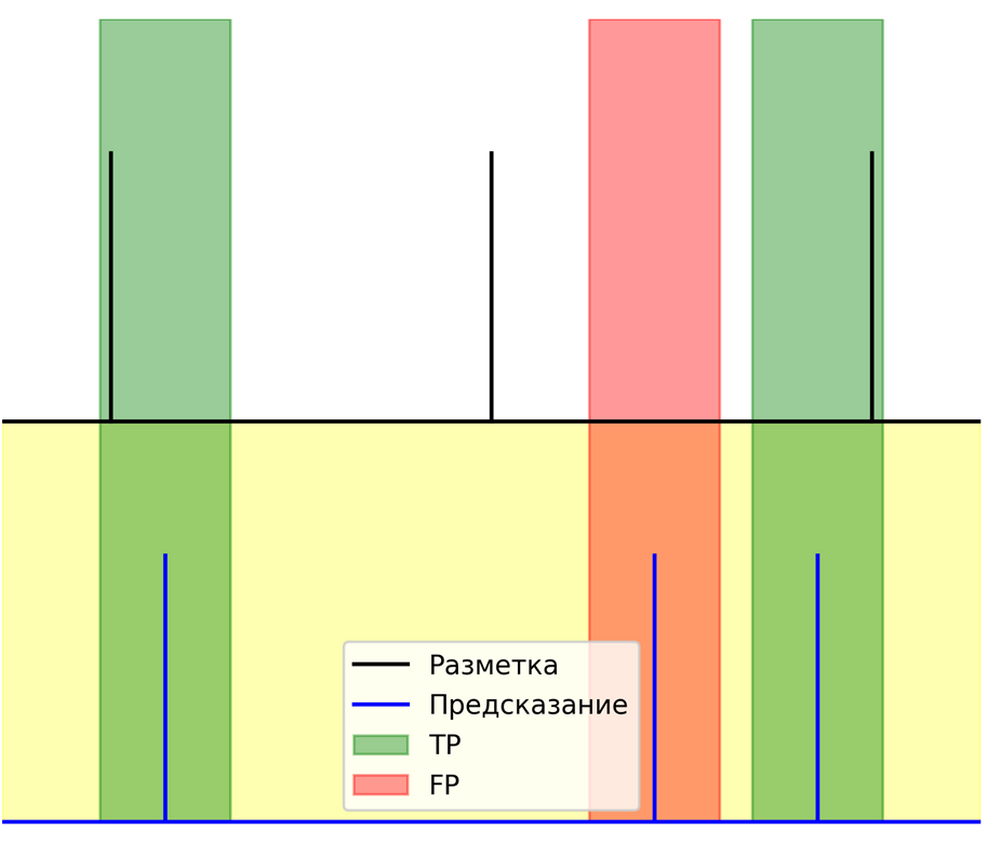
\includegraphics[width=.49\textwidth]{metrics1.png}}
	\subfigure[]{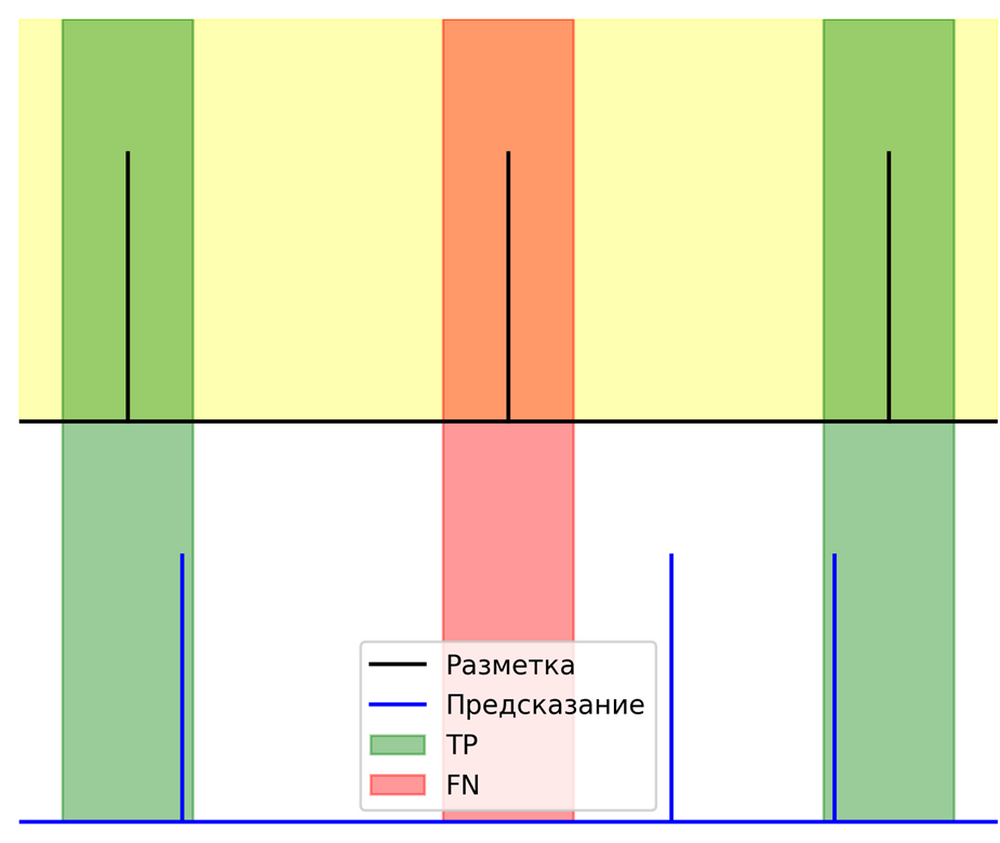
\includegraphics[width=.49\textwidth]{metrics2.png}}
	\caption{(a) Подсчет TP и FP (b) Подсчет FN}
	\label{fig:metrics}
\end{figure}

После подсчета TP, FP и FN по формулам, описанным выше, вычисляется $F_1score$.
